\chapter{A time-series model of foreign affairs: sentiment between nation-states}
\label{chapter:foreign_relations}

\section*{Introduction}

In this chapter we will use the text of newspaper articles to infer a
history of the relationships between different nations.  An assumption
of our work is that the tension between two nations---or a warm and
robust relationship between them---is reflected by the language that
is used to discuss them.  In developing this assumption, we will
discuss two models designed to infer the relationships between pairs
of countries.

\subsection*{Text and latent spaces}
The basic unit of analysis in this chapter will be paragraphs of text
from newspaper articles which discuss pairs of countries.  We choose
paragraphs because they are small enough to have just one or two
concrete ideas but large enough to describe interesting
relationships.

We will use some of the same ideas presented in the last chapter to
model the text of these paragraphs, but we will use concepts from
Chapter 2 to model relationships between pairs of countries.  This
will allow us to model the history of countries over time.  An
advantage of a text-based approach to history is that we can
incorporate information from all articles of a given collection with
modest computational cost.  This means that historians and political
scientists can then search and review thousands of historical
documents at the push of a button---or identify forgotten and
overlooked incidents in history.

An important additional assumption that we will make is that each
nation can be summarized by its position in a latent space, so that
the sentiment between two nations is determined (up to stochasticity)
by the relationship between their positions in this latent space.  By
making this assumption, we will gain two benefits: the ability to
interpret these countries' positions, since they provide statistically
meaningful summaries of these countries' positions; and the ability to
make predictions about the relationships between countries, based on
their latent positions. While the last chapter's Document Influence
Model allowed us to discover themes which evolved over time and individual
documents' influence on these themes, the assumptions we will make in
this chapter will allow us to create a more rich story about the
interaction of specific textual entities---countries---over time.

% We infer sentiment with the supervision of voting on UN resolutions.
% Learning sentiment based on voting patterns provides an objective
% measure of the political goals of different countries.

% Potential idea: can use filtering instead of smoothing to see
% how things look "as they happen".

\subsection*{Organization of this chapter}

In the next two sections we will develop several computational models that
link the text of a news source to the relationships between countries.

We begin with a model which infers these relationships by using using
two sources of labels about the the relationship, or sentiment,
between pairs of countries: expert labels and labels assigned by lay
paid ``workers''.  To design this model, we will develop a set of
spatio-temporal assumptions that allow us to describe the sentiment
between countries by inspecting their relative positions in this
latent space (and, inversely, to interpret their positions based on
observed sentiment).  We will demonstrate that modeling countries in
this way allows us to create a history of foreign relations over time.
Importantly, we will demonstrate that the sentiment inferred from two
very different sources of sentiment labels leads to strikingly similar
measures of inter-state sentiment.

After developing this supervised model, we invert this question and
ask: what sentiment is implied by the text alone of news articles?  To
answer this question, we describe an unsupervised model of the
relationship between countries to qualitatively describe these
relationships.  We then demonstrate a connection between the
unsupervised relationships and the sentiment labels we had used for
the supervised model.


%\section{Foreign relations and their influence on news reporting}
%

\section{A latent-space model of foreign relations}


\section{A supervised model of dyadic sentiment}
\section{A supervised model of dyadic sentiment}

\label{section:foreign_relations_supervised_model}

In the last chapter we described a model for identifying influential
documents.  An important feature of that model was that it was
unsupervised; only after it was fit did we compare the inferred
influence of an article with the number of citations it had recieved.
In this section we will take a more direct approach, fitting a
model with labels \emph{defined} to represent sentiment.

Here will make further assumptions about the object of discussion in
the text. We will assume in particular that each country can be
described by a vector in some latent space.  The relationship between
two countries is then determined (up to stochasticity) by the
relationship between these countries' positions in this latent space
(models that make this assumption are sometimes referred to as latent
space models or spatial models).  A spatial a model provides two
benefits for us. First, it provides interpretability: nations with similar
positions in this latent space tend to interact more positively, while
nations further apart tend to have more tension in their relationship.
A spatial model also allows us to draw on existing work from
multidimensional scaling, which has been used successfully in both
political science \cite{martin:2002,jackman:2001} and social network
modeling \cite{hoff:2002,chang:2009}.

\subsection{Inferring sentiment from text.}
\label{section:text_regression}
When a news source discusses the relationship between these nations,
the author's choice of words $\bm w_d$ reflects the relationship
between the countries.  We model this sentiment with the text of the
article $d$.  Using text regression \cite{kogan:2009}, we model
sentiment using the wordcounts $\bm w_d$ of the article:
\begin{align}
  s_d | \bm w_d, \beta \sim \mathcal{N}( \bm w_d^T \beta, \sigma_W^2 ).
  \label{eq:sentiment_text}
\end{align}
For the purposes of countries' positions in the latent-space model, we
will assume that $\beta$ is observed (we describe how to fit $\beta$
with \myeq{sentiment_text} and human labels in
Section~\ref{section:mturk}).  In fitting $\beta$, we interpret the
distribution of $s_d$ as a Gaussian with a mean which depends on the
text.

\subsection{A temporal model of interaction.}
We formalize the latent space assumption by letting each country $c$
take a position $\bm x_c \in \mathbb{R}^p$ in a space of latent
political sentiment. The relationship between two countries $c_1, c_2$
will be described by a scalar $s_{c_1,c_2} \in \mathbb{R}$.  This
sentiment is determined by the interaction of their positions:
$s_{c_1, c_2} = \mathcal{F}(\bm x_{c_1}, \bm x_{c_2})$, for some
suitable function $\mathcal{F}$.

\begin{figure}
  \center
  \vspace{-55pt}
  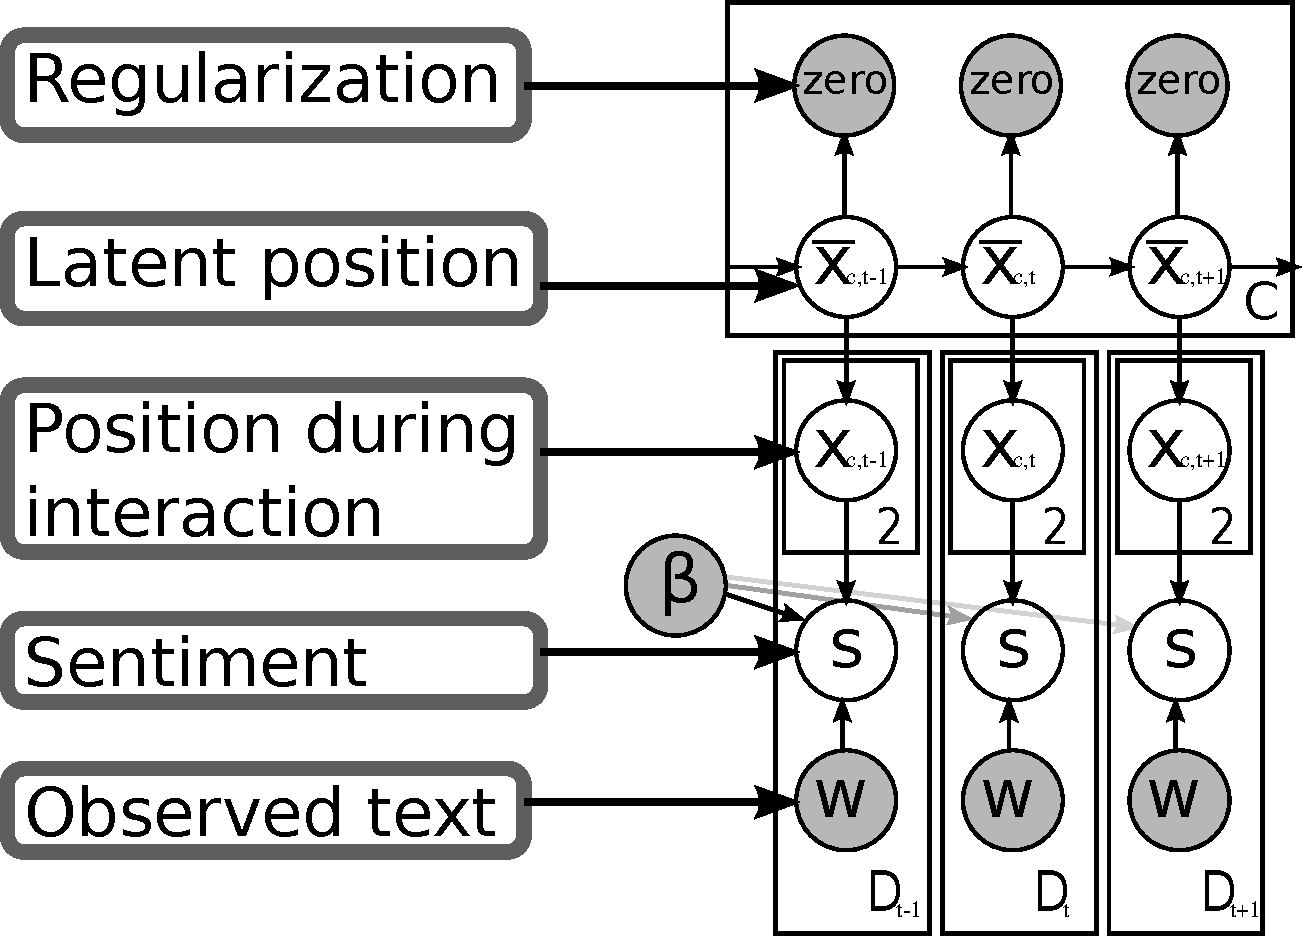
\includegraphics[width=0.5\textwidth]{chapter_foreign_relations/figures/countries_gm.pdf}
  \caption{A time-series model of countries' interactions.
    Pseudo-observations of ``zero'' are added for regularization.
    Amazon Mechanical Turk labels are used to fit $\beta$, which is
    used to infer unobserved sentiments.}
  \label{figure:gm}
\end{figure}


Foreign relations are not static; nations' alliances and preferences
change over time with the evolution of economies, technology, and
culture.  Therefore we make this a fully temporal model by
allowing each country's mean position $\bar x_{c,t}$ to drift over
time with the Markov transition
\begin{align}
  \bar x_{c,t} | \bar x_{c,t-1} \sim \mathcal{N}(\bar x_{c,t-1}, \sigma_{\mbox{\tiny chain}}^2),
\end{align}
as shown in Figure~\ref{figure:gm}. At any time $t$, state $c_1$ may interact with state $c_2$ in the following way:
\begin{align}
  x_{c_1,d} \sim \mathcal{N}(\bar x_{c_1, t}, \sigma_D^2) \nonumber \\
  x_{c_2,d} \sim \mathcal{N}(\bar x_{c_2, t}, \sigma_D^2) \nonumber \\
  s_d := x_{c_1,d}^T x_{c_2,d}, \label{eq:sentiment_space}
\end{align}
where we interpret $s_d$ as the sentiment between $c_1$ and $c_2$ as
reflected by article $d$.  When $c_1$ and $c_2$ are similar (as
measured by their inner product), their sentiment $s_d$ will be
positive; if they are dissimilar, their sentiment will be negative.
More extreme values indicate stronger sentiment.

For the purposes of countries' positions in the latent-space model,
however, we will use the symmetry of the Gaussian to model text as if
it were conditioned on sentiment: $\mathcal{N}(s_d | \bm w_d^T \beta,
\sigma_w^2) = \mathcal{N}( \bm w_d^T \beta | s_d, \sigma_W^2 )$.  This
allows us to reconcile \myeq{sentiment_text} and
\myeq{sentiment_space}, so that the distribution of sentiment
conditioned on text and countries' positions is:
\begin{align}
  p(s_d | \bm w_d, \beta, x_{c_1,d}, x_{c_2,d}) & \propto
  \mathcal{N}(\bm w_d^T \beta | s_d, \sigma_W^2 )
  \mathcal{N}(x_{c_1,d} | \bar x_{c_1, t}, \sigma_D^2)
  \mathcal{N}(x_{c_2,d} | \bar x_{c_2, t}, \sigma_D^2) \nonumber \\
  & \hspace{20pt} \mbox{ such that } s_d = \mathcal{F}(x_{c_1,t},
  x_{c_2,t}) \nonumber \\
  & = 
  \mathcal{N}(\bm w_d^T \beta |
    \mathcal{F}(x_{c_1,t}, x_{c_2,t}), \sigma_W^2 )
  \mathcal{N}(x_{c_1,d} | \bar x_{c_1, t}, \sigma_D^2)
  \mathcal{N}(x_{c_2,d} | \bar x_{c_2, t}, \sigma_D^2).
\end{align}

% In addition, a UN resolution may come up for vote at any time.  States
% cast a vote based on their current positions:
% \begin{align}
% x_{c_1,d} \sim N(\bar x_{c_1, t}, \sigma_D^2) \nonumber \\
% p(v_{cr}) = \sigma(x_{c_2, t} b_r + a_r) \nonumber \\
% \end{align}

% \begin{wrapfigure}{r}{0.4\textwidth}
%   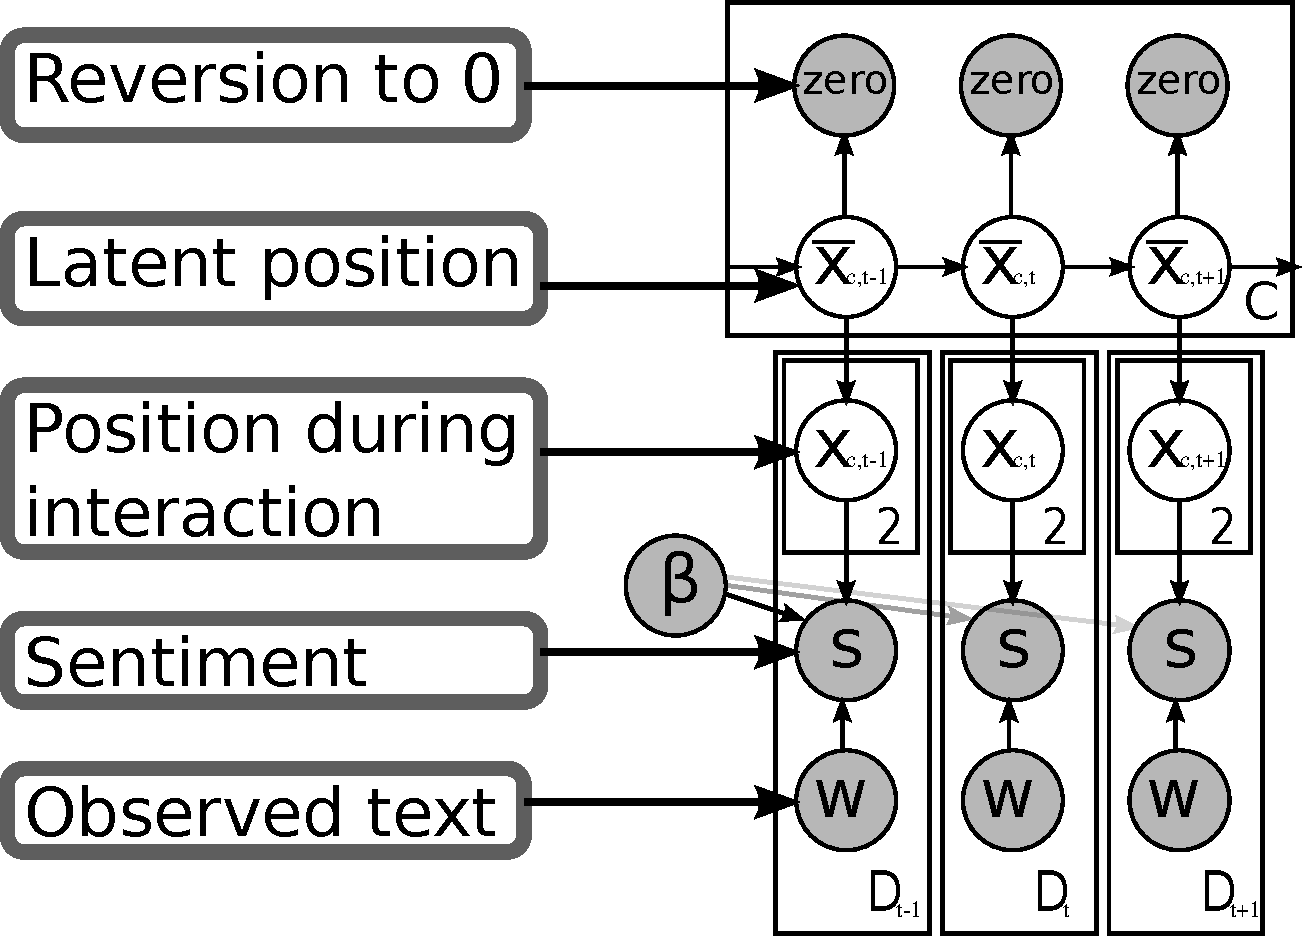
\includegraphics[width=0.4\textwidth]{figs/countries_gm.pdf}
%   \caption{The full time-series model of interaction by countries.
%     The large plate shows replication of a Markov chain for each
%     country.  Certain countries interact at each epoch -- possibly
%     multiple times -- with sentiment $s$.}
%   \label{fig:countries_by_ip}
% \end{wrapfigure}

\paragraph{A brief comment on notation.} Before proceeding to
inference and the experimental validation of this model, we pause to
summarize our use of notation.  In this chapter, we will use notation
flexibly when it is convenient.  The typical unit of discussion will
be the $d$th document occurring at time $t$.  The $d$th document
discusses two countries, $c_1$ and $c_2$; these define a tuple $(\{
c_1, c_2 \}, d, t)$ (where the set $\{ c_1, c_2 \} = \{ c_2, c_1 \}$).
We will generally use $d$ to index documents, $t$ or $s$ to index
time, and $c$ to index a country.  When document $d$ is given, we may
refer to its time $t_d$ (which is unique) or to the two interacting
countries as $c_{d,1},c_{d,2}$ or $c_1,c_2$.  Alternatively, we may
refer to the documents in which a country $c$ appears as $d_{c,1},
\ldots, d_{c,1}$.  For example, we may index the variable
$x_{(c_1,d,t)}$ variously as $x_{c_{d,1}}$ or $x_{d,1}$, or even $x_c$
if the context is clear. The sentiment between two countries might be
described as $s_d$, $s_{c_1,c_2}$, $s_{d,t}$, or $s_{c_1,c_2,d,t}$.

\subsection{Related work}

% Democracy, Political Similarity, and International Alliances, 1816-1992
% Brian Lai
% Dan Reiterb
% Department of Political Science, Emory University
Spatial models such as Item Response Theory (IRT) have been developed
over the past century by quantitative social scientists for analyzing
behavior.  While much of this work has been used to model
parliamentary voting behavior, these techniques have also been used to
model voting in the UN General Assembly. Gartzke et al., for example,
use these votes and alliance models to study the nations' affinities
\cite{gartzke:1998}.

These models have been developed for dyadic data more fully in network
models such as the latent space model \cite{hoff:2002,sarkar:2005}, in
which the probability of a link between two nodes is a function of
their latent-space distance.  The qualitative relationship of
entities' dyadic relationships has been more fully developed with text
by the relational topic model, which uses free text to model the
relationship between actors in an unsupervised setting
\cite{chang:2009}.
% Supervised topic models


% Affinity of states dataset: 
% Fading Friendships (working paper)
% Alliances, Affinities and the Activation of International Identities∗
% Erik Gartzke†
% Alex Weisiger‡
% 7 March 2011

\subsection{Inference}
We fit the \emph{MAP} objective of this probabilistic model.  This has
the benefit of both clean exposition and simple implementation, and it
can be interpreted as a form of unregularized variational inference.
We optimize the \emph{MAP} objective in this model using an
expectation maximization (EM) algorithm.

We designed the probabilistic objective to make inference tractable.
For example, the Gaussian distribution of per-document sentiment
variables $x_{c, t} | \bar x_{c,t}$ makes inference for $\bar x_{c,t}$
closed-form.  Countries' per-interaction positions $x_{c_{d,1}, t},
x_{c_{d,2},t} | \bar x_{c_{d,1},t}, \bar x_{c_{d,2}, t}, s_{c_{d1},
  c_{d2}}$ are then fit using gradient ascent.

Our goal in performing EM is to estimate parameters for the model.  Expectation allows us to find a \emph{MaP} estimate by optimizing the lower bound on the data likelihood:
\begin{align}
  \mathcal{L_{x}} \log p(s_d, \bm w, \beta, x)
  % & \propto p(s_d | \bm w, \beta, x, \beta) \\
  & \ge \log \expectq{ \frac{q(\bar x)}{q(\bar x)}
    p(s_d | \bm w, \beta, x, \beta) } \nonumber \\
  & \ge \expectq{ q(\bar x)
    \log \frac{ p(s_d | \bm w, \beta, x, \beta) }{
      q(\bar x)} }
\end{align}

\subsubsection{M Step.} In the M step, we estimate the mean $\bar
x_{c,t} | x_{c_1,1}, \ldots, x_{c_N,T}$ of each country's position
using a modified Kalman filter (modified because it must take into
account all interactions in a given year).  This step differs from a
standard Kalman filter in that we may have no or multiple observations
on any given date.\footnote{We also experimented with
  \emph{pseudo-observations} for each country at each day $t$ with
  mean 0 and variance $\sigma_p^2$.  These observations are a form of
  ``time-series regularization'' and reflect the sense that a lack of
  news is effectively neutral news.  Low values of $\sigma_p^2$ harmed
  performance, and it was best set around $10^6$.}  The prior over the
ends of the chain are standard normal.

\paragraph{Kalman updates.}
The M step seeks the expected value of the mean position $\bar x_c$
for each country $c$ given our estimate of the $D_{c,s}$ interactions
at each time $s=1, \ldots, T$:
\begin{align}
  \arg \max \bar x_{c,t} | x_{c,1,1}, \ldots, x_{c,D_{c,1},1}, x_{c,D_{c,2},2},
  \ldots, x_{c,D_{c,t},T},
\end{align}
for $t=1, \ldots, T$. The optimal value for $\bar x$ can be found with
a modified Kalman smoother \cite{kalman:1960}.  This modified Kalman
smoother requires a forward filter step and a backward filter step.
The forward filter estimates the mean position given all previous
observations (note that we use $x_{c,d,t}$ to describe the position of
country $c$ at time $t$ for interaction $d$:
\begin{align}
  \bar x_{\mbox{\tiny forth},c,t} | \bar x_{\mbox{\tiny forth},c,t-1}, \{ x_{c,d,t-1} \}_{d}
  & \gets \frac{\bar x_{\mbox{\tiny forth},c,t-1} / \sigma_{\mbox{\tiny forth},t-1}^2
    + \sum_{d=1}^{D_{c,t-1}} x_{c,d,t-1} / \sigma_{\mbox{\tiny obs}}^2}
  {1 / \sigma_{\mbox{\tiny forth},t-1}^2 + 1 / \sigma_{\mbox{\tiny obs}}^2} \\
  \sigma_{\mbox{\tiny forth},t}^2
  & \gets \frac{1}{1 / \sigma_{\mbox{\tiny forth},t - 1}^2
    + D_{c,t-1} / \sigma_{\mbox{\tiny obs}}^2} + \sigma_{\mbox{\tiny chain}}^2,
\end{align}
with initial condition $\bar x_{c,0} = 0,
\sigma_{\mbox{\tiny forth},0}^2=10$.  The backward step estimates
the chain's mean given all current and future observations:
\begin{align}
  \bar x_{\mbox{\tiny back},c,t} | \bar x_{\mbox{\tiny back,c,t+1}}, \{ x_{c,d,t} \}_d
  & \gets \frac{\bar x_{\mbox{\tiny back},c,t+1} / \sigma_{t+1}^2
    + \sum_{d=1}^{D_{c,t}} x_{c,d,t} / \sigma_{\mbox{\tiny obs}}^2}
  {1 / \sigma_{\mbox{\tiny back},t-1}^2 + 1 / \sigma_{\mbox{\tiny obs}}^2} \nonumber \\
  \sigma_{\mbox{\tiny back},t}^2
  & \gets \frac{1}{1 / (\sigma_{\mbox{\tiny back},t + 1}^2 + \sigma_{\mbox{\tiny chain}}^2)
    + D_{c,t} / \sigma_{\tiny obs}^2},
\end{align}
with initial conditions $\bar x_{\mbox{\tiny back},c,T} = 0, \sigma_{\mbox{\tiny
    backward},T}^2=10$. The smoothed means---that is, the mean of countries' positions at time $t$ given all observations for all time---are
\begin{align}
  \expectq{\bar x_{c,t}} & = \bar x_{c,t} | x \nonumber \\
  & = \bar x_{c,t} | \bar x_{\mbox{\tiny forth,c,t}}, \bar x_{\mbox{\tiny back,c,t}}, \sigma_{\mbox{\tiny back}}^2, \sigma_{\mbox{\tiny forth}}^2 \nonumber \\
  & = \frac{\bar x_{\mbox{\tiny forth},c,t} / \sigma_{\mbox{\tiny forth},t}^2
    + \bar x_{\mbox{\tiny back},c,t} / \sigma_{\mbox{\tiny back},t}^2}
  {1 / \sigma_{\mbox{\tiny forth},t}^2
    + 1 / \sigma_{\mbox{\tiny back},t}^2}
\end{align}

% x_{c,d,t}
\subsubsection{E Step.} In the E-step, our goal is to infer each
nation's position $x_{c_{d,1}} | \expectq{ \bar{x}_{c,d,t} },
x_{c_{d,2}}, s_d$ during interaction $d$ given its expected mean $\expectq{ \bar
x_{c_{d,1},t_d} }$ and the text $\bm w_d$ describing this interaction,
\emph{and} given the other country's position for this interaction.
We find these positions by gradient ascent on each interaction:
\begin{align}
  & {\arg \max}_{x_{c_{d,1},t}, x_{c_{d,2},t}}
  p(\bm w_d^T \beta | \mathcal{F}(x_{c_{d,1},t}, x_{c_{d,2},t}),
  \expectq{ \bar x_{c_{d,1},t} }, \expectq{ \bar x_{c_{d,2},t} }) \nonumber \\
  & = 
  {\arg \max}_{x_{c_{d,1},t}, x_{c_{d,2},t}}
  p(\bm w_d^T \beta | \mathcal{F}(x_{c_{d,1},t}, x_{c_{d,2},t}), \beta)
  p(x_{c_{d,1},t} | \expectq{ \bar x_{c_{d,1},t} } )
  p(x_{c_{d,2},t} | \expectq{ \bar x_{c_{d,2},t} } ).
\end{align}

\subsection{Empirical studies: comparisons with ground truth}
We now turn to an experimental analysis of this model.  We first
describe the human labels we have used to define sentiment $s_d$
within this model.  We then describe two news archives from which we
have inferred countries' sentiment over time. text in which the
relationships of countries are deto which we applied this model and .
We then turn

\subsection{Sentiment labels $s$}
\label{section:sentiment_models}

To infer the sentiment $s_d$ between two countries, we treat the
corresponding news article as a bag of words and fit text regression
\cite{kogan:2009} to predict the sentiment from the text.  We used two
sources for sentiment labels: Amazon Mechanical Turk and Covariates of
War.  In each case, we fit a text regression which predicted the
sentiment $s_d$ from a training set of text snippets.

\subsection{Datasets and tokenization}

\paragraph{New York Times.}
We fit and evaluate this model over news articles discussing 245
nations and territories from twenty years of the \emph{New York Times}
(NYT).  This collection spanned the years 1987 to 2007, a period which
included both Gulf wars; the collapse of the Soviet Union; the
reunification of Germany; September 11th, 2001; and countless other
world events.

\paragraph{Data preparation.}
We used articles from the Foreign, Business, Financial, and Magazine
desks of the newspaper during this period. We made an important
assumption that the scope of foreign sentiment discussion is at the
level of a paragraph.  We therefore used the subset of paragraphs
which discuss exactly two nations as ``documents'' $d$, a collection
of 257,472 paragraphs from 1987 to 2007.  We then defined a vocabulary
to be those words which appeared at least twenty times in the
collection, in no more than 40\% of documents, and in at least 0.1\%
of documents.

This resulted in a vocabulary of 5958 words, mentioned by 40,356
paragraphs. We randomly selected 80\% (32,249) distict paragraphs from
this set as training examples and used the remaining examples to
evaluate our model.

We next labeled our training examples with both human reviewers and
expert labels, representing opposite ends of the extreme.

\subsubsection{Amazon Mechanical Turk labels}
\label{section:mturk}

\emph{Amazon Mechanical Turk} (AMT) is a crowdsourcing platform which
provides a \emph{requestor} (the author of this thesis) with access to
thousands of \emph{workers} who perform simple tasks over the
Internet.  Although the requestor can use tests to ensure that workers
are high-quality, these workers are typically not experts.

\begin{figure*}
  \setlength\fboxsep{0pt}
  \setlength\fboxrule{0.5pt}
  \center \fbox{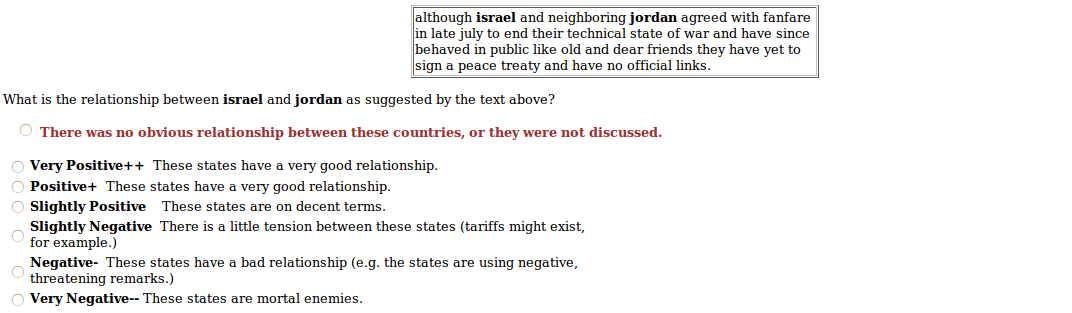
\includegraphics[width=1.0\textwidth]{chapter_foreign_relations/figures/mturk_screenshot.png}}
  \label{figure:mechanical_turk_sample}
  \small\caption{A screenshot of a Mechanical Turk labeling task.
    Sometimes relationships may be complicated; both raters gave this
    example a score of ``slightly positive''.}
  \normalsize
\end{figure*}

To fit the model, we asked \emph{Amazon Mechanical Turk} raters to
rate the sentiment between two nations mentioned in the text of a
paragraph on the scale -5 (mortal enemies), $\ldots$, 5 (very good
relationship). We illustrate a rating task (as seen by a Mechanical
Turk worker) in \myfig{mechanical_turk_sample}.

Raters were asked to review a random subset of 3607 paragraphs from
the original collection.  Before fitting the model, we manually
disqualified eight raters (out of 85) who consistently performed
poor ratings.

With all rated paragraphs which were not in the test set, we fit the
coefficients $\bm \beta$ of the text regression discussed in
Section~\ref{section:model}.  This coefficient was then treated as
constant in the joint model in Figure~\ref{figure:gm} to allow us to
infer sentiment from the words of all 32,249 training paragraphs.  We
illustrate the $\bm \beta$ inferred from Mechanical Turk-labeled
paragraphs in \myfig{fr_example_betas} (left).

\subsubsection{Expert labels: Correlates of War}
\label{section:correlates_of_war}

We also used a combined set of expert labels based on the Correlates of War \cite{sarkees:2010} and Issue Correlates of War \cite{hensel:2001}.
\begin{itemize}
  \item The \emph{Correlates of War} project ``seeks to facilitate the
    collection, dissemination, and use of accurate and reliable
    quantitative data in international relations''
    \cite{cow_webpage:2012}, and it provides labels describing the
    relationships between pairs of countries from 1823 to 2003.
    At-war is a binary relationship (either countries are at war, or
    they are at peace). We used a list of CoW inter-state wars
    (version 4.0) from 1823 to 2003 of inter-state wars
    \cite{sarkees:2010}.
  \item The \emph{Issue Correlates of War} project ``is a research
    project that is collecting systematic data on contentious issues
    in world politics'' \cite{icow_webpage:2012}, and they provide
    expert labels on a variety of inter-state conflicts that \emph{do
      not require militarized conflict}.  However, these issue label
    do require documented evidence of contention between states; such
    issues include maritime and territorial disputes.
    \cite{icow_webpage:2012,hensel:2001}.
\end{itemize}

We combined these datasets by treating two countries as having a
rating of -5 if they are at war from the Correlates of War codes and
-1 if there is any contentious issue between the countries in the
Issue Correlates of War.\footnote{These values were selected to
  correspond roughly to the Mechanical Turk labels.}.  All other pairs
of countries were treated as having a rating of 0.1.  As before, we
fit the text regression parameters $\beta$ using these labels on the
training set and evaluated countries' ratings on the test dataset. We
illustrate $\bm \beta$ fit to CoW-labeled paragraphs in
\myfig{fr_example_betas} (left).

\begin{figure}
  \begin{tabular}{cc}
    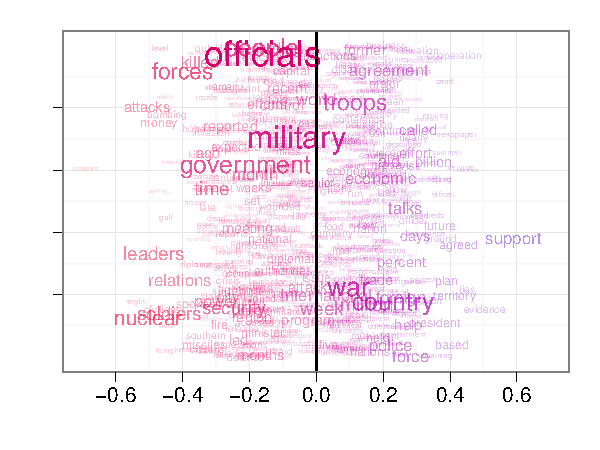
\includegraphics[width=0.4\textwidth]{chapter_foreign_relations/figures/mturk_sample_words.pdf} &
    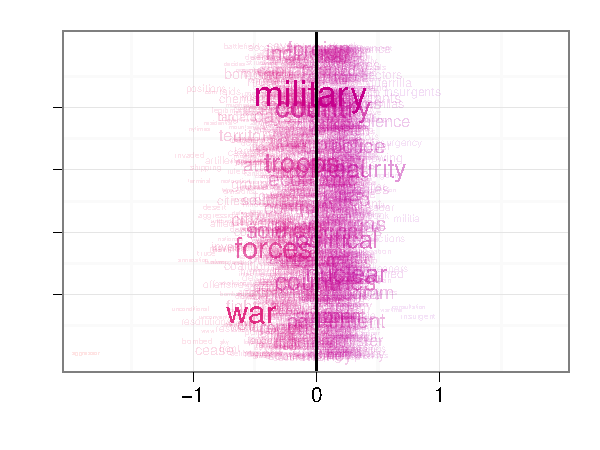
\includegraphics[width=0.4\textwidth]{chapter_foreign_relations/figures/cow_sample_words.pdf} \\
    \end{tabular}
  \caption{Coefficients $\beta_w$ for selected words $w$ fit on text
    labeled by Amazon Mechanical Turk workers (left) and Correlates of
    War data (right). Coefficients fit from Mechanical Turk labels are
    more clearly separated than those fit to Correlates of War labels;
    this is likely due to explicit positive sentiment in that dataset.
    The $x$-axis is $\beta$, and the $y$-axis is used for display (it
    corresponds to no variable).  Size of each word is proportional to
    $\sqrt{\mbox{frequency}}$, and color corresponds to $\beta$.}
  \label{figure:fr_example_betas}
\end{figure}

\subsubsection{Casual vs. expert labels}
The CoW represent a data source which is fairly different from
Mechanical Turk ratings. In the NYT dataset, CoW ratings and
Mechanical Turk ratings were correlated at $\sigma=0.196$.  To
see why this was the case, we give several examples:
\begin{itemize}
  \item $s_{d,\mbox{AMT}} = 1, s_{d,\mbox{CoW}}=-5$. \emph{as an
    indication of the dangers the damage occurred in waters where
    military spokesmen said no mines had been suspected before but
    where a \textbf{saudi} officer said today that some 22 were later
    found. \textbf{iraq}i mines widely deployed} \cite{cushman:1991}
  \item $s_{d,\mbox{AMT}} = -5, s_{d,\mbox{CoW}}=0.1$ \emph{not since
    the grim old days of the cold war have relations between the
    \textbf{united states} and russia been quite as problematic as they
    are this weekend on the eve of president clinton's visit for
    celebrations marking the 50th anniversary of the allied victory in
    europe in world war ii.} \cite{apple:1995}
\end{itemize}

The first of these examples outlines a limitation in the ratings we
obtained: a single paragraph is sometimes too small a unit of
discussion.  This meant Mechanical Turk workers likely missed the
larger context of the article about the Gulf war (including the title,
\emph{War in the Gulf: Sea Mines; Allied Ships Hunt Gulf for Iraqi
  Mines}).

The second example represents a limitation of both data sources.  The
two Mechanical Turk ratings of -5 were clearly too strong, as the
countries are not at war; but AMT workers likely based their rating in
part on the reference to World War II (worker instructions deserve a
rating of -3 or, possibly -1).  In addition, however, the United
States and Russia were not at War and had no official, documented
conflicts at this time.  This means that this sentiment was not
reflected in the CoW labels -- which defaulted to 0.1.

\label{section:experiments}

\subsubsection{Results}
 \begin{figure}
  \begin{tabular}{ccc}
    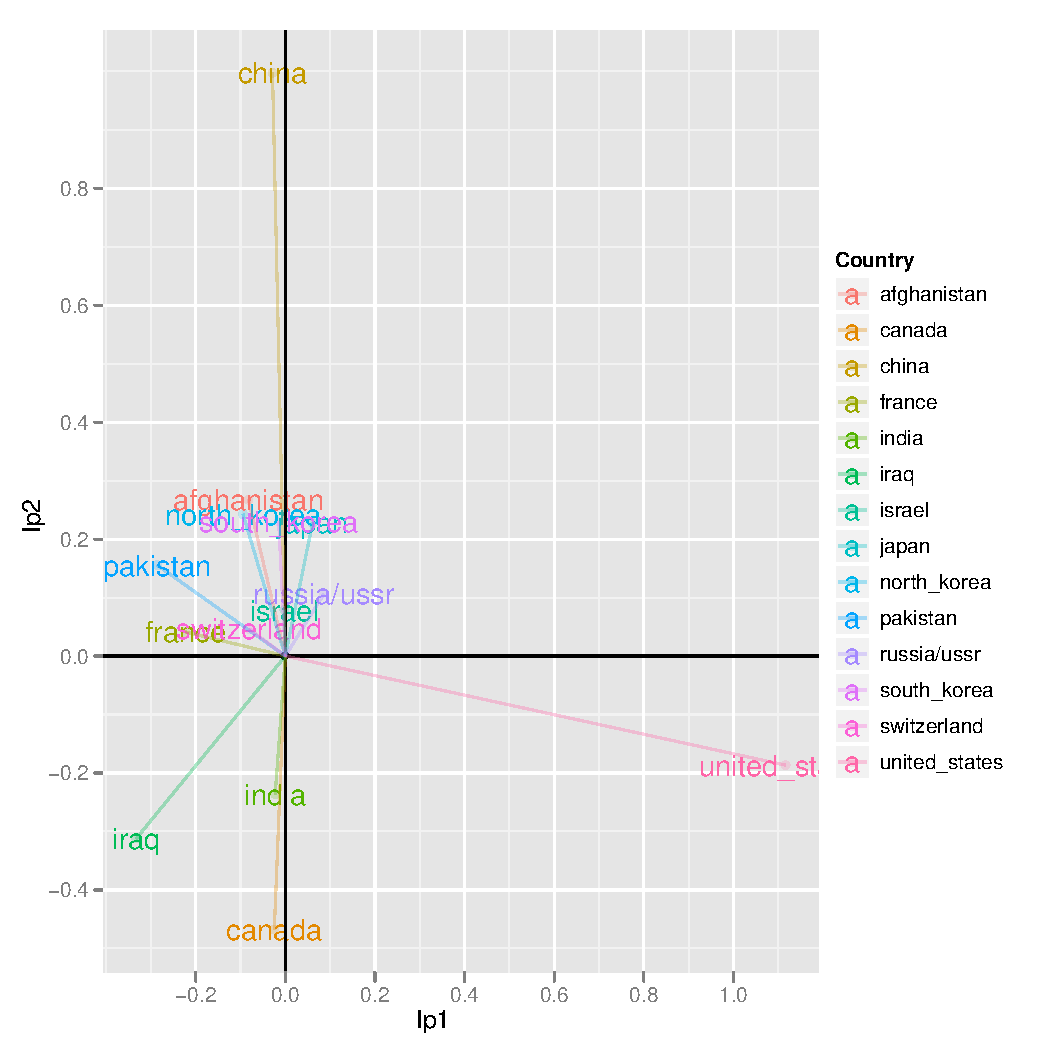
\includegraphics[width=0.33\textwidth]{chapter_foreign_relations/figures/002_countries_by_ip_1987.pdf} &
    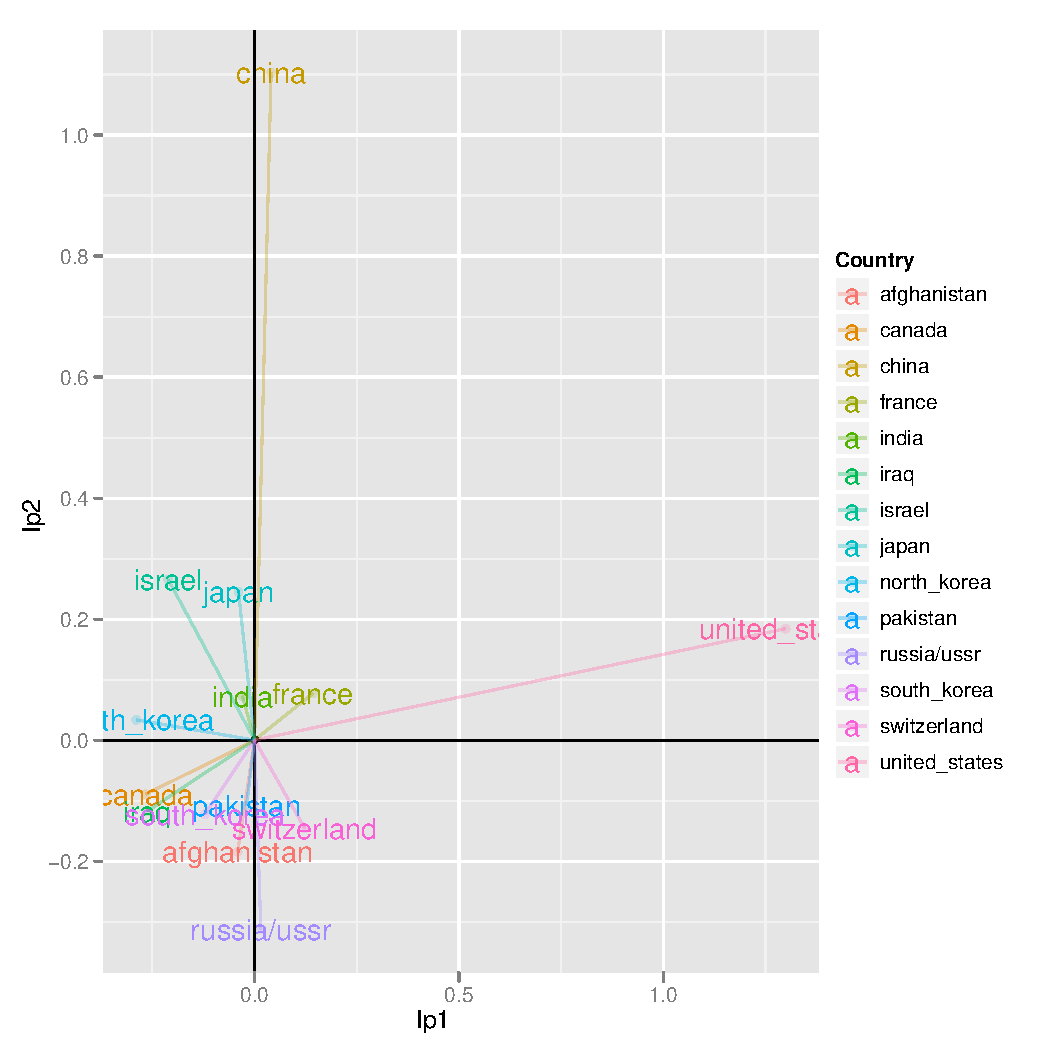
\includegraphics[width=0.33\textwidth]{chapter_foreign_relations/figures/002_countries_by_ip_2007.pdf} &
    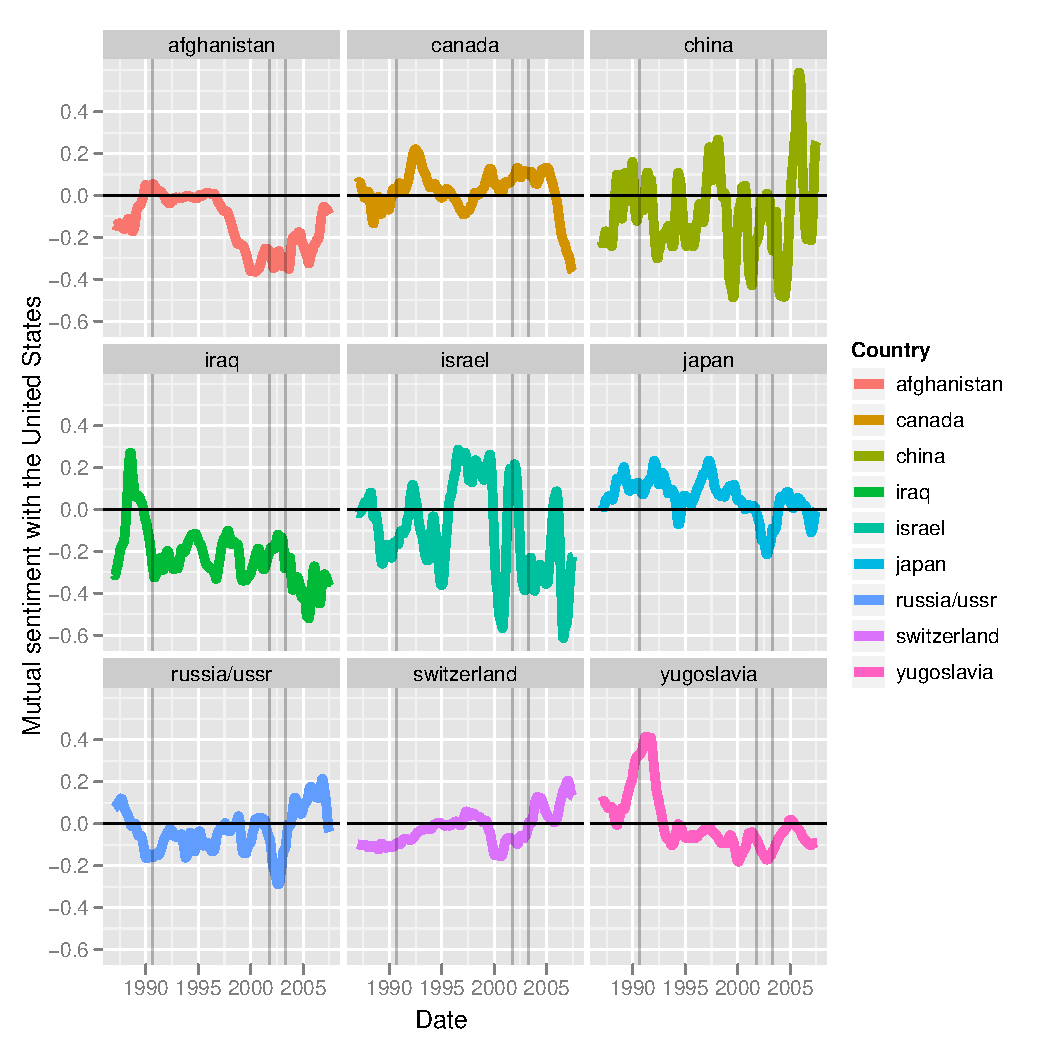
\includegraphics[width=0.33\textwidth]{chapter_foreign_relations/figures/002_us_vs_everyone.pdf} \\
    (a) & (b) & (c) \\
  \end{tabular}
  \caption{
    (a) Example positions of selected countries in the latent space of national sentiment, in 1987. Sentiment is given by the inner product between two vectors.
    (b) Example positions of selected countries in 2007.
    (c) Mutual sentiment $s = \bar x_{c, \cdot}^T \bar x_{\mbox{\small us}, \cdot}$ with the United States over time. The two Iraq wars and September 11th, 2001 are marked.
  }
  \label{figure:figures}
\end{figure}

\subsection{Results}

\paragraph{Prediction.}
For two nations $c_1$ and $c_2$ mentioned together at time $t$, we
predict their sentiment to be $\tilde s_{c_1, c_2} = \bar x_{c_1,t}
\bar x_{c_2, t}$.  Based on this estimate, the average squared error
for heldout nations is 2.32 ($R^2=0.51$), considerably better than a
baseline of text regression, which had means-squared-error $5.53$; for
comparison, average \emph{inter-rater squared error} -- the minimum
theoretically possible given the set of Mechanical Turk ratings -- was
$1.77$, and the square of the difference \emph{between} raters was
$7.11$.  We also found that using ``pseudo observations'' with even
modest observation variance improves predictive performance; these
results are summarized in Table~\ref{figure:sse_test}.

\paragraph{Static latent space.}
We first evaluate the latent-space assumption that countries'
interactions can be summarized by their positions in a latent space.
For this, we used a simplified model of sentiment, in which documents'
mean positions $\bar x_c, y_c$ are fixed, and that the sentiment is
drawn from .

We tested this assumption for both a distance and inner-product link
function, with intercepts and without intercepts.  We find that the
the inner-product assumption $\bar x_{c_1}^T \bar x_{c_2}$ alone is
poor because it provides no natural way to model mischief-prone
countries well.  If the inner-product model is endowed with intercepts
$y_{c_1}, y_{c_2}$, however, it becomes a top-performer.

Both the inner product and distance link functions perform best when
they are able to use intercepts and when they have many dimensions: we
evaluated the models with up to 9 dimensions, and they TODO(sgerrish), modeling articles' sentiment at 0.32.

\paragraph{The benefit in adding Markov drift.}
We can improve the predictive power of this model by adding a time
dimension, allowing $\bar x_c$ to drift over time for each country
$c$.  We illustrate these results in (bottom).

The inner product model again performed poorly, often worse than the
baseline model.  In this case, the seven-dimensional distance link
function performed better than any other model, and adding per-country
intercepts $y_c$ significantly \emph{hurt} the model's performance.

The better performance of these models under a time-series assumption
provides support for the argument that countries' relationships change
over time, and that these relationships are observed through the news
cycle.

\paragraph{Improvement due to zero-reversion regularization}
We can improve the predictive power of this model by adding a time
dimension, allowing $\bar x_c$ to drift over time for each country
$c$.  We illustrate these results in (bottom).

The inner product model again performed poorly, often worse than the
baseline model.  In this case, the seven-dimensional distance link
function performed better than any other model, and adding per-country
intercepts $y_c$ significantly \emph{hurt} the model's performance.

The better performance of these models under a time-series assumption
provides support for the argument that countries' relationships change
over time, and that these relationships are observed through the news
cycle.

\paragraph{Static latent space.}

\begin{figure}
  \begin{tabular}{|c|c|c|c|c|c|c|c|}
   \hline
  Link $\mathcal{F}(\bm x_{c_1}, y_{c_1}, \bm x_{c_2}, y_{c_2})$ & & & & & & \\
  \hline
  \textbf{Dimension of $\bm x$} & 0 & 1 & 2 & 3 & 4 & 5 & 6 & 7 & 8 & 9 \\
  \hline
  $y_{c_1} + y_{c_2}$ & 0.0964 & - & - & - & - & - & - & - & - & - \\
  \hline
  $\bm x_{c_1}^T \bm x_{c_2}$
  & 0.1036 & 0.1013 & 0.1050 & 0.1038 & 0.1033 & 0.1025 & 0.1018 & & & \\
  \hline
  $y_{c_1} + y_{c_2} + \bm x_{c_1}^T \bm x_{c_2}$
  & 0.0964 & 0.0943 & 0.0940 & 0.0936 & 0.0935 & 0.0934 & 0.0934 & & & \\
  \hline
  $-\log(||\bm x_{c_1} - \bm x_{c_2}||_2^2 + 1)$
  & 0.1036 & 0.1037 & 0.0978 & 0.0957 & 0.0951 & 0.0947 & 0.0943 & & & \\
  \hline
  $y_{c_1} + y_{c_2} -\log(||\bm x_{c_1} - \bm x_{c_2}||_2^2 + 1)$
  & 0.0964 & 0.0949 & 0.0943 & 0.0938 & 0.0939 & 0.0937 & 0.0936 & & & \\
  \hline
  mean($\{s_d\}_d$) & 0.1036 & - & - & - & - & - & - & & & \\
  \hline
  \end{tabular}
  \vspace{30pt}
  \begin{tabular}{|c|c|c|c|c|c|c|c|}
   \hline
  Link $\mathcal{F}(\bm x_{c_1}, y_{c_1}, \bm x_{c_2}, y_{c_2})$ & & & \\
  \hline
  \textbf{Dimension of $\bm x$} & 0 & 1 & 2 & 3 & 4 & 5 & 6 \\
  \hline
  $y_{c_1} + y_{c_2}$ & 0.0964 & - & - & - & - & - & - \\
  \hline
  $\bm x_{c_1}^T \bm x_{c_2}$
  & 0.1036 & 0.1013 & 0.1050 & 0.1038 & 0.1033 & 0.1025 & 0.1018 \\
  \hline
  $y_{c_1} + y_{c_2} + \bm x_{c_1}^T \bm x_{c_2}$
  & 0.0964 & 0.0943 & 0.0940 & 0.0936 & 0.0935 & 0.0934 & 0.0934 \\
  \hline
  $-\log(||\bm x_{c_1} - \bm x_{c_2}||_2^2 + 1)$
  & 0.1036 & 0.1037 & 0.0978 & 0.0957 & 0.0951 & 0.0947 & 0.0943 \\
  \hline
  $y_{c_1} + y_{c_2} -\log(||\bm x_{c_1} - \bm x_{c_2}||_2^2 + 1)$
  & 0.0964 & 0.0949 & 0.0943 & 0.0938 & 0.0939 & 0.0937 & 0.0936 \\
  \hline
  mean($\{s_d\}_d$) & 0.1036 & - & - & - & - & - & - \\
  \hline
\end{tabular}
   \caption{Mean-squared error of text sentiment inferred with a
     static sentiment model across 20 years of \emph{New York Times}
     articles. An inner-product model with four dimensions (plus
     intercepts) performs best.}
\end{figure}

Nations' positions are illustrated in Figure~\ref{figure:figures}.
Figures~\ref{figure:figures}(a,b) show nations' relative positions
and interactions for a two- dimensional model; heldout error slightly
increased for higher dimensions. The United States' relationship with
Iraq (see Figure~\ref{figure:figures}(c)) serves as an excellent
example of this model in action; the relationship between these
nations degrades during both the Gulf War and the invasion of Iraq
following September 9th, 2001.  Israel's relationship with the United
States demonstrates one of the model's downfalls: while Israel is
considered a close ally of the United States, the raters' 95 ratings
of these nations' mentions had mean 0.12 and standard deviation
2.65.  Because the model is only as good as its ratings, the nations
appear to have a rocky relationship.

% > a = read.csv("../../data/v4/v4-doc-training_samples.csv", as.is=TRUE, header=FALSE)


  %  We then evaluate perplexity
 % \begin{align}
 %   \mbox{perp}_d & = \mathcal{E_{\hat D}} \log p(w | \bar x_{d_{c1}}
 %     \bar x_{d_{c2}} ) \\
 %     & = \frac{1}{N} \sum_N \sum_{W_{d_n}}
 %     \log p(w | \bar x_{d_{c1}} \bar x_{d_{c2}} ) \\
 % \end{align}

% \subsubsection*{Bivariate change point detection}
% In addition to identifying the latent positions of nations over
% time, we can pinpoint periods of great change or upheaval.  Sudden
% changes in a nation's position is an indication of newsworthy events
% in its history; simultaneous changes in two nations' positions is an
% indication that they are both taking part in these newsworthy events.

% The task of identifying sudden changes in a time-series is known as
% change point detection.  Change point detection is frequently
% addressed by simple univariate significance tests.  We consider
% changes in the statistic $\bar s_{c1,c2} := \bar x_{c1} \bar x_{c2}$
% (see Equation~\ref{figure:sentiment}).  Because $\bar s_{c1,c1}$ may
% be change significantly when either $x_{c_1}$ or $x_{c_2}$ changes, we
% search for simultaneous significant changes in $\bar x_{c_1}$, $\bar
% x_{c_2}$, and $\bar s_{c1,c2}$ (Note that $\mathcal{E}[s_{c1,c2}] \neq
% \bar s_{c1,c2}$; we compute $\bar s_{c1,c2}$ out of convenience.



\section{Unsupervised relationships between countries}
\section*{Unsupervised relationship mining}

% There are some limitations to modeling sentiment in a supervised way.
%   - Don't have explicit sentiment labels
%   - The interactions between countries is better described
%     by a dimension orthogonal to "war".
%     - Trade
%     - Culture and society

The preceding approach has limitations, however.  First, sentiment
labels measure only one kind of interaction: whether countries are at
war or peace.  In reality, relationships between countries may be
characterized in many ways, some of which are independent of whether
countries are at war.  For example, the relationship between coutries
may be characterized by trade in goods, or by the exchange of culture
and society. Another limitation to a supervised sentiment model is
that labels of the sentiment between countries may be unavailable or
limited, or (as we saw before), the labels may be noisy.

% in this section, we will describe a model which will allow us to discover
% unsupervised relationships
%   - We will use a modul much like RTM
%   - RTM is ...
In this section we will describe a model for inferring relationships
between countries in an unsupervised fashion.  This model serves as an
alternative to the model in the last section in that it requires no
explicit labels of the relationship between pairs of countries.
Instead it infers a qualitative relationship between countries -- a
relationship which we can attempt to interpret post-hoc.  The
significance of this approach is that it infers a relationship between
countries based more on the discussion of these countries than
explicit labels.  Particularly, if there is a relationship which has
been overlooked by historians, then we might be able to learn it.

In the remainder of this section we will outline a probabilistic model
for inferring sentiment between pairs of countries.  We will outline
the key assumptions of this model -- first, a language model inspired
by the \emph{Networks Uncovered by Bayesian Inference} model
\citep{chang:2009nubbi}; and second, a spatial model of dyadic
relationships. We will then describe inference for this model, and
finally provide an empirical analysis of this model.

\subsection{A model of unsupervised foreign relations}
% The assumptions are as follows:
%   - Each country is associated with a background distribution
%   - Each interaction is described by:
%     - words related to either country
%     - miscellaneous words
%     - words about the relationship between the two countries
In the supervised foreign relations discourse model, our aim is to
characterize the relationship between two countries by inspecting the
language used to describe them.  This model comprises two pieces: a
language model for describing the language used to discuss countries;
and a time-series spatial model to describe the relationship between
pairs of countries.  We will begin by outlining the spatial sentiment
model, which will be familiar to readers from the last section.  We
then describe the language model, which is similar to LDA.  We then
describe how these two models are connected.

\subsubsection*{Dynamic spatial model}
The assumptions for interaction between countries in the unsupervised
model are similar to those we used in the supervised model from the
last section.  Each country is characterized by a position $\bar
x_{ct}$ which drifts over time in some latent space $\mathbb{R^d}$.
Pairs of countries interact according to the dyadic relationship
\begin{align}
  x_{c_1,d} | \bar x_{c_1,t} & \sim \mathcal{N}(\bar x_{c_1, t}, \sigma_s^2) \nonumber \\
  x_{c_2,d} | \bar x_{c_2,t} & \sim \mathcal{N}(\bar x_{c_2, t}, \sigma_s^2) \nonumber \\
  s_d | x_{c_1,d}, x_{c_2,d}, r_{c_1,d}, r_{c_2,d} & = \log( || x_{c_1,d} - x_{c_2,d} ||_2^2 + 1), \nonumber \\
  \kappa_d | s_d & \sim \sigma(s_d),
\end{align}
where each country $c$ has an additional intercept $r_c$ and
$\sigma(s)$ is the logistic function $\frac{\exp(s)}{1 + \exp(s)}$.
We illustrate this graphically in \myfig{dynamic_dyadic_chain}.  As in the
last section, we use the extra variables $x$ instead of $\bar x$ for
computational convenience because we can estimate the time-series
average $\bar x$ in closed form with a Kalman smoother.

Also as before, we attach an intercept $\bar r_{c_2}$ to each country
to model each country's typical interaction style.  This gives us the augmented model
\begin{align}
  r_{c_1,d} | \bar r_{c_1} & \sim \mathcal{N}(\bar r_{c_1}, \sigma_r^2) \nonumber \\
  r_{c_2,d} | \bar r_{c_2} & \sim \mathcal{N}(\bar r_{c_2}, \sigma_r^2) \nonumber \\
  s_d | x_{c_1,d}, x_{c_2,d}, r_{c_1,d}, r_{c_2,d} & = \log( || x_{c_1,d} - x_{c_2,d} ||_2^2 + 1)  + r_{c_1} + r_{c_2} \nonumber \\
  \kappa_d | s_d & \sim \sigma(s_d)
\end{align}
We illustrate this sentiment model graphically in \myfig{dynamic_dyadic_chain}.

The sentiment parameter $\kappa_d$ will become important when we link
this sentiment model to text.  Intuitively, if two countries are far
apart in the latent space at time $t$, we expect that $\kappa$ is more
likely to be 1 when they interact.  Otherwise, $\kappa$ is more likely
to be 0.  As we develop the language model, we will use this random
variable to decide which topic is used to describe the pair of countries.

\subsubsection*{Binary Relational language model}
We incorporate text using a mixed-membership language model similar to
LDA.  Recall that in LDA, each word comes from a specific topic.  In
our model, which we dub the \emph{binary relational language model},
we assume that the words describing a pair of countries come from
topics about those countries.

\paragraph{A mixture of four topics.} To be concrete, consider a document discussing Iran and the United
States.  We assume that each word in this document will serve one of
four roles:
\begin{enumerate}
  \item It discusses the U.S. only,
  \item It discusses Iran only,
  \item It discusses the relationship between the U.S. and Iran. \label{foreign_relations:relationship}
  \item It is a ``filler'' word, providing little contribution to the discussion. \label{foreign_relations:filler}
\end{enumerate}
The first two roles for a word are self-explanatory.  The relationship in
(\ref{foreign_relations:relationship}) above could be any type of
relationship -- the goal of this section is of course to discover the
relationships in a collection of documents about these
countries.  The ``filler'' words in
(\ref{foreign_relations:filler}) above are those words found in any document
-- stopwords, for example -- that are unrelated to either country or
the relationship between them.

We therefore keep $(N_c + 2 + 1)$ topics---topics $\beta_{C,1},
\ldots, \beta_{C,{N_c}}$ for each of the $N_c$ countries, exactly two
sentiment topics $\beta_{S,0}, \beta_{S,1}$, and a single, global
background topic $\beta_{B0}$ \citep{chemudugunta:2009}.  We assume,
as in LDA, that a document about the United States and Iran is a
mixture of topics; in contrast to LDA, however, we constrain this
document's topics to be exactly the four topics enumerated above:
$\beta_{C,\mbox{\tiny Iran}}$, $\beta_{C,\mbox{\tiny United States}}$,
$\beta_{B,0}$, and either $\beta_{S,0}$ or $\beta_{S,1}$ (we describe
below how to make the choice between $\beta_{S,0}$ and $\beta_{S,1}$).
A document about Hungary and Germany, in contrast, would be a mixture
of the topics $\beta_{C,\mbox{\tiny Germany}}$, $\beta_{C,\mbox{\tiny
    Hungary}}$, $\beta_{B,0}$, and either $\beta_{S,0}$ or
$\beta_{S,1}$.

Once these topics are fixed for a document, the language model
proceeds as with LDA for each word: each word in the document comes
from one of four topics, with probability for topic $k$ proportional
to the topic mixture $\expect \theta_k$.  We illustrate this model
graphically in \myfig{binary_relational_language_model}.  Note that we
keep the topic mixture $\theta$ global instead of local to each
document because the topics are already very constrained.

\subsubsection{Determining the sentiment topic: connecting dyadic sentiment and text}

Up to now the dyadic sentiment model and the language model have been
developed independently.  We connect the two models by using the
binary sentiment parameter $\kappa_d$ to index the sentiment topic for
a document: document $d$ takes topic $\beta_{S,\kappa_d}$ for its
sentiment topic.\footnote{We also make a small adjustment to ensure
  that the model converges to a reasonable mode.  There are two main
  components of this model: a language model and a sentiment model. We
  introduce a parameter $\nu \sim \mathbb{N(0, 100)}$ and per-document
  parameters $\nu_d \sim \mathbb{R}(\nu, 0.001)$ and define the binary
  sentiment $\kappa_d \sim \sigma(s_d \nu_d)$.}
% determine the sentiment topic based on $k$.
In other words, if two countries are far apart in the latent space,
then when they interact in document $d$, this interaction is likely to
be negative (i.e., $\kappa_d = 1$, and the language used to describe
their relationship will come from topic $\beta_{S, 1}$.  If they were
instead close together in this latent space, the language used to
describe their relationship would come from topic $\beta_{S, 0}$.

We can now specify the generative model of a document language, given
the sentiment $\kappa_d$ for each interaction between countries.  We
begin by specifying the global topics.
\begin{enumerate}
\item First, draw topics:
  \begin{enumerate}
  \item For nation $c=1, \ldots, C$:
    \begin{itemize}
    \item Draw topic $\beta_{\mbox{C},c} \sim \mbox{Dir}(1, \ldots, 1)$.
    \end{itemize}
  \item Draw background topic $\beta_{\mbox{B},0} \sim \mbox{Dir}(1, \ldots, 1)$.
  \item Draw positive-interaction topic $\beta_{\mbox{S},0} \sim \mbox{Dir}(1, \ldots, 1)$
  \item Draw negative-interaction topic $\beta_{\mbox{S},1} \sim \mbox{Dir}(1, \ldots, 1)$
\end{enumerate}

\item Next, draw the global topic mixture $\theta \sim \mbox{Dir}(1, 1, 1, 1)$.

\item Finally, draw documents. \\
For document $d=1, \ldots, D$, each representing interactions between pairs of countries $c_{d_1},c_{d_2}$:
  \begin{enumerate}
    \item Draw sentiment index $\kappa_d \sim \sigma(s_d)$
    \item For word $n = 1, \ldots, N_d$:
    \begin{itemize}
      \item Draw $z_{n} \sim \mbox{Mult}(\theta_d$).
      \item Switch($z_n$):
      \begin{itemize}
        \item If $z_n = (1, 0, 0, 0)$, draw $w_n \sim \beta_{\mbox{C},c_{d_1}}$.
        \item If $z_n = (0, 1, 0, 0)$, draw $w_n \sim \beta_{\mbox{C},c_{d_2}}$.
        \item If $z_n = (0, 0, 1, 0)$, draw $w_n \sim \beta_{\mbox{B},0}$.
        \item If $z_n = (0, 0, 0, 1)$, draw $w_n \sim \beta_{\mbox{S},\kappa_d}$.
      \end{itemize}
    \end{itemize}
  \end{enumerate}
\end{enumerate}
We illustrate the combined model in
\myfig{dynamic_dyadic_chain_binary_relational_language_model}.

\subsubsection{Related work}
The binary relational language model is founded on ideas discussed by
several recent models.  Chang et al. developed a model to describe the
relationships between ``entities'' (e.g., countries) with a similar
assumption of entity-specific and relationship-specific topics
\citep{chang:2009nubbi}.  For concreteness, we describe their work in
the context of our work, by using ``country'' where they used the
abstract term ``entity''.  In Chang et al.'s \emph{Networks Uncovered
  by Bayesian Inference} (Nubbi) model, each country had its own
country-specific topic, which was active when that country is
discussed.  An additional mixture of topics was then used to describe
the relationship between countries.  Nubbi was then be used to infer
relationships between countries that have been tagged in a collection
of text documents.

Nubbi inferred relationships between countries by finding similar
topic weights between documents. In contrast, we use sentiment to
select between topics, with an ``upstream'' model in which actors are
embedded in a latent space. This idea of merging topics at different
levels of a hierarchy has also been explored by
\cite{chemudugunta:2009}.  Neither of these approaches included a
switch variable for selecting between topics.

The idea of associating language with sentiment has been explored in
considerable detail lately.  Some of the most successful supervised
approaches handle this with regression methods such as text regression
\citep{kogan:2009}.

Supervised topic models \citep{blei:2008} offer a fully probabilistic
generative model of documents which have an attached label.  A key
assumption behind supervised topics is that the model can learn topics
that capture the underlying sentiment.  Supervised topic models do
this by assuming that the distribution of documents' sentiment
parameters $s_d$ are fully specified given their words' topic indices
$\bm z_d$ and regression coefficients $p(s_d | \bm z_d, \bm \eta)$.
This requires that $p(s_d | \bm w_d, \bm \eta, \bm \beta)$ they are
fully specified given the text of documents and $\eta$. This means
that the topics learned by a standard LDA algorithm will differ from
those learned by a supervised LDA algorithm, because they adjust to
explain documents' sentiment.

The unsupervised sentiment model is similar to supervised LDA in that
the topics adjust as the underlying sentiment parameter $s_d$ differs.
In contrast to supervised topics, we assume an inverted conditional
independence: words of two documents are conditionally independeqnt
given the document's and other model parameters: $p(\bm w_d | s_d,
\beta)$, while supervised LDA assumes that sentiment is conditionally
independent given words and regression coefficients $\bm \eta$.

\begin{figure}
  \center
  \begin{tabular}{lm{2.5in}lm{2.5in}}
    \begin{tabular}{c}
      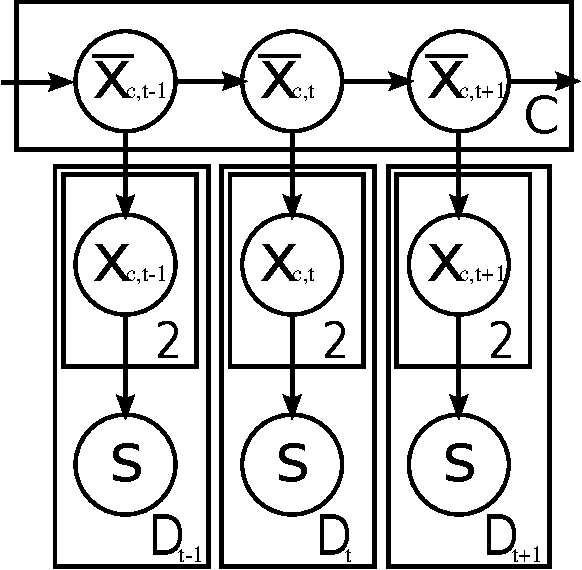
\includegraphics[width=0.26\textwidth]{chapter_foreign_relations/figures/countries_gm_no_text.pdf} \\ (A) \vspace{50pt} \\
      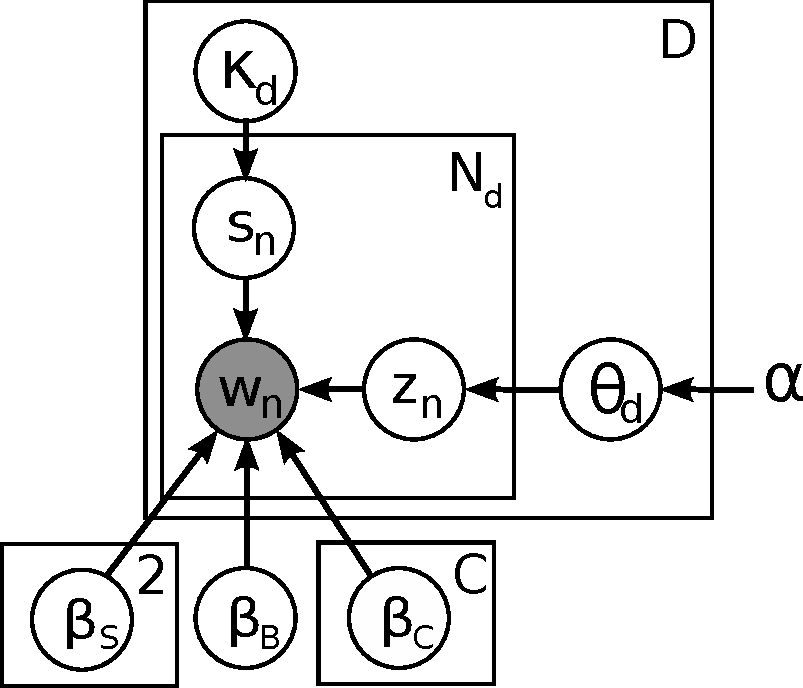
\includegraphics[width=0.35\textwidth]{chapter_foreign_relations/figures/fr_lda_gm.pdf} \\ (B) \\
    \end{tabular}
    &
    \begin{tabular}{c}
    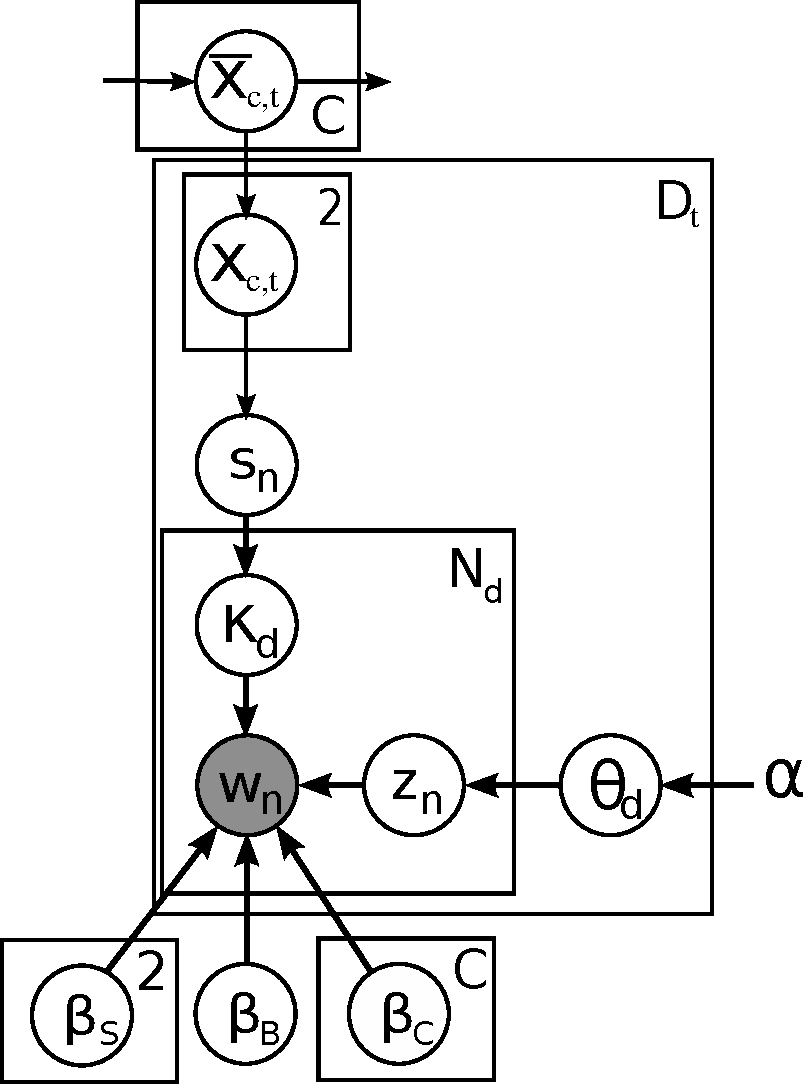
\includegraphics[width=0.35\textwidth]{chapter_foreign_relations/figures/countries_gm_unsupervised_all.pdf} \\ (C) \\
    \end{tabular}
  \end{tabular}
  \caption{The dynamic sentiment model (A), a binary mask
    mixed-membership language model (B), and the full unsupervised
    foreign relations model (C) (which is a combination of (A) and
    (C).  In (B) and (C), we assign each country its own topic
    $\beta_{C,\cdot}$.  Interactions between countries are
    characterized by sentiment $s_d$, which is reflected in the
    sentiment topic $\beta_{S,\kappa_d}$.  The background topic
    $\beta_B$ is provided to ``soak up'' background noise.}
  \label{fig:dynamic_dyadic_chain}
  \label{fig:binary_relational_language_model}
  \label{fig:dynamic_dyadic_chain_binary_relational_language_model}
\end{figure}

\subsection{Inference}
As before, we only observe a collection $\{ (\bm w_d, c_{d,1},
c_{d,2}) \}_{d \in D}$ of interactions between countries.  Each of
these interactions takes the form of a vector of wordcounts $\bm w_d$
and a pair of countries interacting.  To perform an empirical analysis
with this model, we must estimate the latent positions of countries
and the latent topics associated with documents.  These are described
by the hidden random variables $\bar x_c, \theta$, and $\beta$.
We accomplish this with posterior inference, which will provide us
with an estimate of the distribution $p(\bar x_c, \theta, \beta |
\{ (\bm w_d, c_{d,1}, c_{d,2}) \}_{d \in D})$.

We fit this model with \emph{maximum a posteriori} (MAP) inference,
which has the benefit of a simpler derivation than variational
inference.  As the reader may recall, the MAP estimate is
\begin{align}
  \hat x_c, \hat \theta, \hat \beta
  = & \arg \max_{\bar x_c, \theta, \beta} p(\bar x_c, \theta, \beta | \{ (\bm w_d, c_{d,1}, c_{d,2}) \}_{d \in D}) \nonumber \\
  = & \arg \max_{\bar x_c, \theta, \beta} p(\bar x_c, \theta, \beta, \{ (\bm w_d, c_{d,1}, c_{d,2}) \}_{d \in D}). \label{equation:fr_unsupervised_map_likelihood}
\end{align}

Deriving the algorithm for MAP estimation requires expanding the full
likelihood objective, lower-bounding this objective, and maximixing
the lower bound with respect to the parameters.  We have designed the
model in such a way that updates can be performed by a combination of
exact coordinate ascent on each parameter (or its expectation), with
the exception of countries' mean position $\hat x_{c_{d,1}, c_{d,2}}$
during interactions.

The lower bound on the likelihood uses the expectations
$\expect{\kappa_d}$ and $\expect{z_n}$.  This means that each
interaction is manifested as a mixture $\expect{\kappa_d}$ of
sentiment, and the observed words are treated as mixtures $\expect{\bm
  z_d}$ of topics.  We estimate countries' mean positions $\bar \hat
x$ using a Kalman filter \citep{kalman:1960} as in the last section.
This inference step is exactly as in the last section.


\paragraph{Countries' per-interaction positions $x_{c_{d,1}, c_{d,2}}$.}
As in the last section, we infer countries' positions during an
interaction by gradient ascent on the objective with respect to their
positions $x_{c_{d,1}, c_{d,2}}$.

\paragraph{Estimating topics $\beta_{C, \cdot}, \beta_{S, \cdot}$, and $\beta_{B}$.}
The update for topics is similar to that in LDA.  In both cases, we
aggregate the sufficient statistics and normalize during an M-step.
We also use Laplace smoothing by adding pseudo counts of
$0.1$ to these statistics.

\paragraph{Estimating $\expect{\kappa}$ and $\expect{z_n}$.}
During inference, we compute the expectations $\expect{\kappa_d}$ and
$\expect{z_n}$, to perform EM.  The goal of performing EM is to optimize the bound
\begin{align}
  \log p(\bm w_d | \bm \beta, s_d)
  & \ge \log \expectq{ \frac{q(\kappa_d, \bm z_d)}{q(\kappa_d, \bm z_d)} p(\bm w_d | \bm \kappa_d, \bm z_d, \bm \beta, s_d) } \\
%  & = \expectq{ \frac{ q(\kappa_d) }{ q(\kappa_d) } \log \frac{ p(\bm w_d | \bm \kappa_d, \bm z_d) }{ q(\kappa_d) } } \\
  & \ge \expectq{ q(\kappa_d, \bm z_d) \log \frac{p(\bm w_d | \bm \kappa_d, \bm z_d, \bm \beta, s_d)}{q(\kappa_d, \bm z_d)} }
\end{align}
on the likelihood of documents, where we specify $q(\bm \kappa_d, \bm
z_d)$ to be the factorized distribution $q(\bm \kappa_d) q(\bm z_d)$
and write the expectations $q(\bm \kappa_{d} = 1) = \expectq{\bm
  \kappa_d}$, $q(\bm z_{dn}=1) = \expectq{(\bm z_{d,n})}$.

Letting $S_0$ and $S_1$ index the sentiment word-topic distributions,
and letting $S$ index the sentiment topic in the topic indicators $z$,
and recalling that the indicator $z_n$ describes word $w_n$, this
update is:
\begin{align}
  \kappa_{d,0} & \propto \sum_{n=1}^{N_d} \beta_{S_0,w_n} \expect{z_{n,S}} \nonumber \\
  \kappa_{d,1} & \propto \exp(s_d) \sum_{n=1}^{N_d} \beta_{S_1,w_n} \expect{z_{n,S}} \nonumber \\
  \expect{\kappa_{d,i}} & = \frac{\kappa_{d,m}} { \sum_k \kappa_{d,m} } \nonumber \\
\end{align}

The update for $\expect{z_{n}}$ is similar.  Again letting $S (S_0,
S_1)$ refer to the sentiment topic indices, and describing the
remaining indices with $C_1, C_2, B$, we have:
\begin{align}
  z_{n,S} & \propto \expect{\theta_{S}} \left( \beta_{S_0,w_n} \expect{\kappa_{d_z, 0}} + \beta_{S_1,w_n} \expect{\kappa_{d_z, 1}} \right) \nonumber \\
  z_{n,k_{c1}} & \propto \expect{\theta_{C_1}} \beta_{C_1,w_n}  \nonumber \\
  z_{n,k_{c2}} & \propto \expect{\theta_{C_2}} \beta_{C_2,w_n} \nonumber \\
  z_{n,k_{b}} & \propto \expect{\theta_{B}} \beta_{B,w_n} \nonumber \\
  \expect{z_{n,i}} & = \frac{ z_{n,i}} { \sum_k z_{n,k} } \label{equation:fr_e_z}
\end{align}

The update for $\expect{\theta_k}$ is similar to $\kappa_{dk}$, but we use sufficient statistics from all documents:
\begin{align}
  \theta_{k} & \propto \sum_{d=1}^D \sum_{n=1}^{N_d} \expect{z_{n,k}} \nonumber \\
  \expect{\theta_{k}} & = \frac{\theta_{k}} { \sum_m \theta_{m} } \nonumber \\
\end{align}

\subsection*{Empirical analysis}

In this section we perform an empirical validation of this model.  We
will provide anecdotal examples, but our particular interest is in
assessing whether the latent space assumption is a meaningful modeling
assumption.  We begin by providing an overview of the qualitative
results of this model.  We follow this with several metrics of
goodness-of-fit.  These metrics are designed to measure how well the
latent-space assumptions improve the language model and how well the
inferred relationships correspond to third-party metrics of sentiment.

For this analysis, we used the \emph{New York Times}
(NYT).  The NYT corpus included xxxx articles
from which we isolated xxxx paragraphs which mentioned exactly two
countries. There were 87 distinct countries mentioned in these
paragraphs.  We defined a vocabulary of size xxxx by removing words
appearing in fewer than xxx\% of documents or more than xxx\% of
documents.  We split these paragraphs into a set of xxxx training
documents and xxxx test documents.

% \paragraph{XXX.}  The xxx corpus included xxxx articles from which we
% isolated xxxx paragraphs which mentioned exactly two countries. There
% were xxx distinct countries mentioned in these paragraphs.  We defined
% a vocabulary of size xxxx by removing words appearing in fewer than
% xxx\% of documents or more than xxx\% of documents.  We split these
% paragraphs into a set of xxxx training documents and xxxx test documents.

\subsubsection*{Topics}
We first summarize a set of topics inferred by the unsupervised
sentiment model to the entire NYT corpus.
\mytab{fr_unsupervised_topics} lists the most-likely words
from sample of topics fit to these twenty years of articles.

\paragraph{State-specific topics $\beta_{C,\cdot}$.}  The
state-specific topics describe words used when one of these countries
is mentioned in text.  Many of these topics are intuitive: ``oil''
shows up in the Iran topic, and ``drug'' is the top word in the Mexico
topic.  As these countries are mentioned in a major U.S. news source,
the topics are sometimes biased toward ideas specific to the
U.S. relationship with these countries (for example, ``border'' and
``traffickers'' in the Mexico topic).  The U.S. topic contains phrases
specific to policy and leadership.

While these topics are intuitive, they serve little role in analyzing
this collection.  From a modeling perspective, they serve as a
``sponge'' to explain away words commonly used to describe a country,
especially when those words might otherwise be interpreted to refer to
a specific relationship.

\paragraph{An economics/military dichotomy.}
The sentiment topic, on the other hand, is particularly telling.
Again using the convention that $\kappa_d=1$ indicates \emph{negative}
sentiment between countries, the negative-sentiment topic
$\beta_{S,1}$ matches our intuition: it contains words typically
associated with conflict: \emph{military, officials, soldiers, killed,
  troops}, and \emph{police} are among the top words. On the other
hand, the words most likely in the supplementary topic $\beta_{S,0}$
are associated more with economics: \emph{million, percent, people,
  billion, oil}, and \emph{officials}.

Are these words the same words that tend to be associated with expert
labels of sentiment?  The answer is yes.  To quantify this, we used
coefficients from the text regression fit to Mechanical Turk ratings
in the last section.  Among the top 12 words in this topic (shown in
\mytab{fr_unsupervised_topics}), we estimated the average coefficient
learned in the supervised sentiment model.  The average coefficient
for these terms was -0.225, which is less than the mean 0.007 of the
entire vocabulary ($p < 0.02$ by a 2-sample $t$-test).  The mean of
the per-word sentiment $\beta$ for this collection of words was at the
$20th$ percentile of words in the vocabulary.

This contrasts with the top words in either the complementary topic
$\beta_{S,0}$ or the background topic $\beta_{B}$.  The top words in
these topics had respective mean sentiments $\beta$ of $-0.11, -0.08$.
Neither of these was not statistically noteworthy ($p=0.15,0.16$).

% million & military \\
% percent & officials \\
% people & soldiers \\
% billion & killed \\
% oil & troops \\
% officials & police \\
% country & forces \\

% What do the topics look like?
%  background topic?

\begin{figure}
%         Country
% 2   united_states
% 3            iran
% 4           japan
% 8          canada
% 13          china
% 17           iraq
% 24        ireland
% 31  great_britain
% 243            X1
%                                                                                             Topics
% 2   officials,military,official,policy,political,support,government,meeting,leaders,administration
% 3                             nuclear,war,program,weapons,officials,arms,oil,hostages,gulf,uranium
% 4               trade,economic,countries,officials,market,economy,world,military,companies,markets
% 8                      trade,country,free,province,border,agreement,speaking,percent,law,officials
% 13               rights,human,trade,relations,officials,nuclear,visit,political,democracy,economic
% 17               forces,weapons,military,troops,officials,government,security,war,chemical,country
% 24                     police,people,province,peace,killed,political,bomb,control,violence,killing
% 31          officials,government,authorities,intelligence,week,people,minister,colony,time,country
% 243             war,political,officials,country,people,military,international,peace,confirmed,week
% mexico: drug,officials,border,law,enforcement,traffickers,agents,police,authorities,trade,cocaine,illegal
  \center
\begin{tabular}{|c|c|}
  \hline
  \textbf{Background topic ($\beta_{B}$)} \\
  \hline
  war \\
  political \\
  officials \\
  country \\
  people \\
  military \\
  international \\
  peace \\
  confirmed \\
  week \\
  following \\
  government \\
  \hline
\end{tabular}
\hspace{30pt} \begin{tabular}{|cc|}
  \hline
  \textbf{Economics topic ($\beta_{S,0}$) vs.} &
  \textbf{Military topic ($\beta_{S,1}$)} \\
  \hline
  million & military \\
  percent & officials \\
  people & soldiers \\
  billion & killed \\
  oil & troops \\
  officials & police \\
  country & forces \\
  money & people \\
  aid & attack \\
  government & border \\
  companies & near \\
  military & air \\
  \hline
\end{tabular}
\\
\vspace{30pt}
\begin{tabular}{|c|c|c|}
  \hline
  \textbf{Pakistan ($\beta_{C,\mbox{\tiny Pakistan}}$)} &
  \textbf{Mexico ($\beta_{C,\mbox{\tiny Mexico}}$)} &
  \textbf{Israel ($\beta_{C,\mbox{\tiny Israel}}$)} \\
% Iran: nuclear,war,program,weapons,officials,arms,oil,hostages,gulf,uranium
% China: rights,human,trade,relations,officials,nuclear,visit,political,democracy,economic
% india: nuclear,countries,border,weapons,tests,talks,nations,military,state,territory,war,militants
% pakistan: nuclear,weapons,military,officials,terrorism,border,war,government,aid,support,countries,militants
% mexico: drug,officials,border,law,enforcement,traffickers,agents,police,authorities,trade,cocaine,illegal
% israel: peace,territories,occupied,talks,officials,negotiations,agreement,state,settlement,security,settlements,violence
  \hline
  nuclear & drug & peace \\
  weapons & officials & territories \\
  military & border & occupied \\
  officials & law & talks \\
  terrorism & enforcement & officials \\
  border & traffickers & negotiations \\
  war & agents & agreement \\
  government & police & state\\
  aid & authorities & settlement \\
  support & trade & security \\
  \hline
\end{tabular}
\vspace{10pt}
\begin{tabular}{|c|c|c|}
  \hline
  \textbf{United States ($\beta_{C,\mbox{\tiny United States}}$)} &
  \textbf{Iran ($\beta_{C,\mbox{\tiny Iran}}$)} &
  \textbf{China ($\beta_{C,\mbox{\tiny China}}$)} \\
% Iran: nuclear,war,program,weapons,officials,arms,oil,hostages,gulf,uranium
% China: rights,human,trade,relations,officials,nuclear,visit,political,democracy,economic
% india: nuclear,countries,border,weapons,tests,talks,nations,military,state,territory,war,militants
% pakistan: nuclear,weapons,military,officials,terrorism,border,war,government,aid,support,countries,militants
% mexico: drug,officials,border,law,enforcement,traffickers,agents,police,authorities,trade,cocaine,illegal
  \hline
  officials & nuclear & rights \\
  military & war & human \\
  official & program & trade \\
  policy & weapons & relations \\
  political & officials & officials \\
  support & arms & nuclear \\
  government & oil & visit \\
  meeting & hostages & political \\
  leaders & gulf & democracy \\
  administration & uranium & economic \\
  \hline
\end{tabular}
\caption{Per-country topics ($\beta_{C,\cdot}$), a background topics ($\beta_{B,0}$), and the two interaction topics ($\beta_{S,0}, \beta_{S,1}$).}
\label{fig:fr_unsupervised_topics}
\end{figure}

\subsubsection*{Quantitative evaluation}
\paragraph{Perplexity}
% comparison with LDA, for a variety of topics.
% comparison with 
\paragraph{Sentiment}

\paragraph{Relationship between sentiment and third-party sentiment}




\subsection{Posterior inference}

\subsection{Supervised sentiment analysis}

  - Introduce Amazon Mechanical Turk
  - Describe supervised relationships and the model of sentiment from 

\subsection{Unsupervised sentiment analysis}

 - Describe relational topic model

\subsection{Relation to ideal points inferred from the UN General Assembly}

\section*{Conclusions}
